\documentclass[tikz,border=8pt]{standalone}

\usepackage{amsmath,amssymb}
\usetikzlibrary{arrows.meta,backgrounds,calc,fit,positioning}

\definecolor{ink}{HTML}{17212B}
\definecolor{muted}{HTML}{5B6773}
\definecolor{panel}{HTML}{F7F9FA}
\definecolor{panelborder}{HTML}{DCE2E7}
\definecolor{datafill}{HTML}{E8EDF1}
\definecolor{encoderfill}{HTML}{C9E7F1}
\definecolor{encoderline}{HTML}{26799B}
\definecolor{actorfill}{HTML}{D5EBD7}
\definecolor{actorline}{HTML}{347A3D}
\definecolor{dynamicsfill}{HTML}{F8DEB9}
\definecolor{dynamicsline}{HTML}{A96512}
\definecolor{metricfill}{HTML}{E8DDF2}
\definecolor{metricline}{HTML}{70459A}
\definecolor{lossfill}{HTML}{FFF4DB}
\definecolor{loopfill}{HTML}{FBE0DE}
\definecolor{loopline}{HTML}{C6463D}

\tikzset{
  every node/.style={font=\sffamily, text=ink},
  route/.style={-{Latex[length=2.6mm,width=1.8mm]}, line width=0.8pt, draw=ink,
                rounded corners=2pt},
  shared route/.style={route, dashed, draw=encoderline},
  inner route/.style={route, draw=loopline, line width=1.2pt},
  data/.style={draw=muted, fill=datafill, rounded corners=2pt, align=center,
               minimum height=9mm, inner sep=3mm, font=\sffamily\small},
  encoder/.style={draw=encoderline, fill=encoderfill, rounded corners=2pt,
                  align=center, inner sep=3.5mm, font=\sffamily\small},
  actor/.style={draw=actorline, fill=actorfill, rounded corners=2pt,
                align=center, inner sep=3.5mm, font=\sffamily\small},
  dynamics/.style={draw=dynamicsline, fill=dynamicsfill, rounded corners=2pt,
                   align=center, inner sep=3.5mm, font=\sffamily\small},
  metric/.style={draw=metricline, fill=metricfill, rounded corners=2pt,
                 align=center, inner sep=3.5mm, font=\sffamily\small},
  loss/.style={draw=dynamicsline, fill=lossfill, rounded corners=2pt,
               align=left, inner sep=3.5mm, font=\sffamily\small},
  loop/.style={draw=loopline, fill=loopfill, rounded corners=2pt,
               align=center, inner sep=3.5mm, font=\sffamily\small},
  pair/.style={draw=muted, fill=white, rounded corners=2pt, align=center,
               inner sep=2.5mm, font=\sffamily\small},
  note/.style={font=\sffamily\scriptsize, text=muted, align=left},
  lane title/.style={font=\sffamily\bfseries\small, anchor=west},
}

\begin{document}
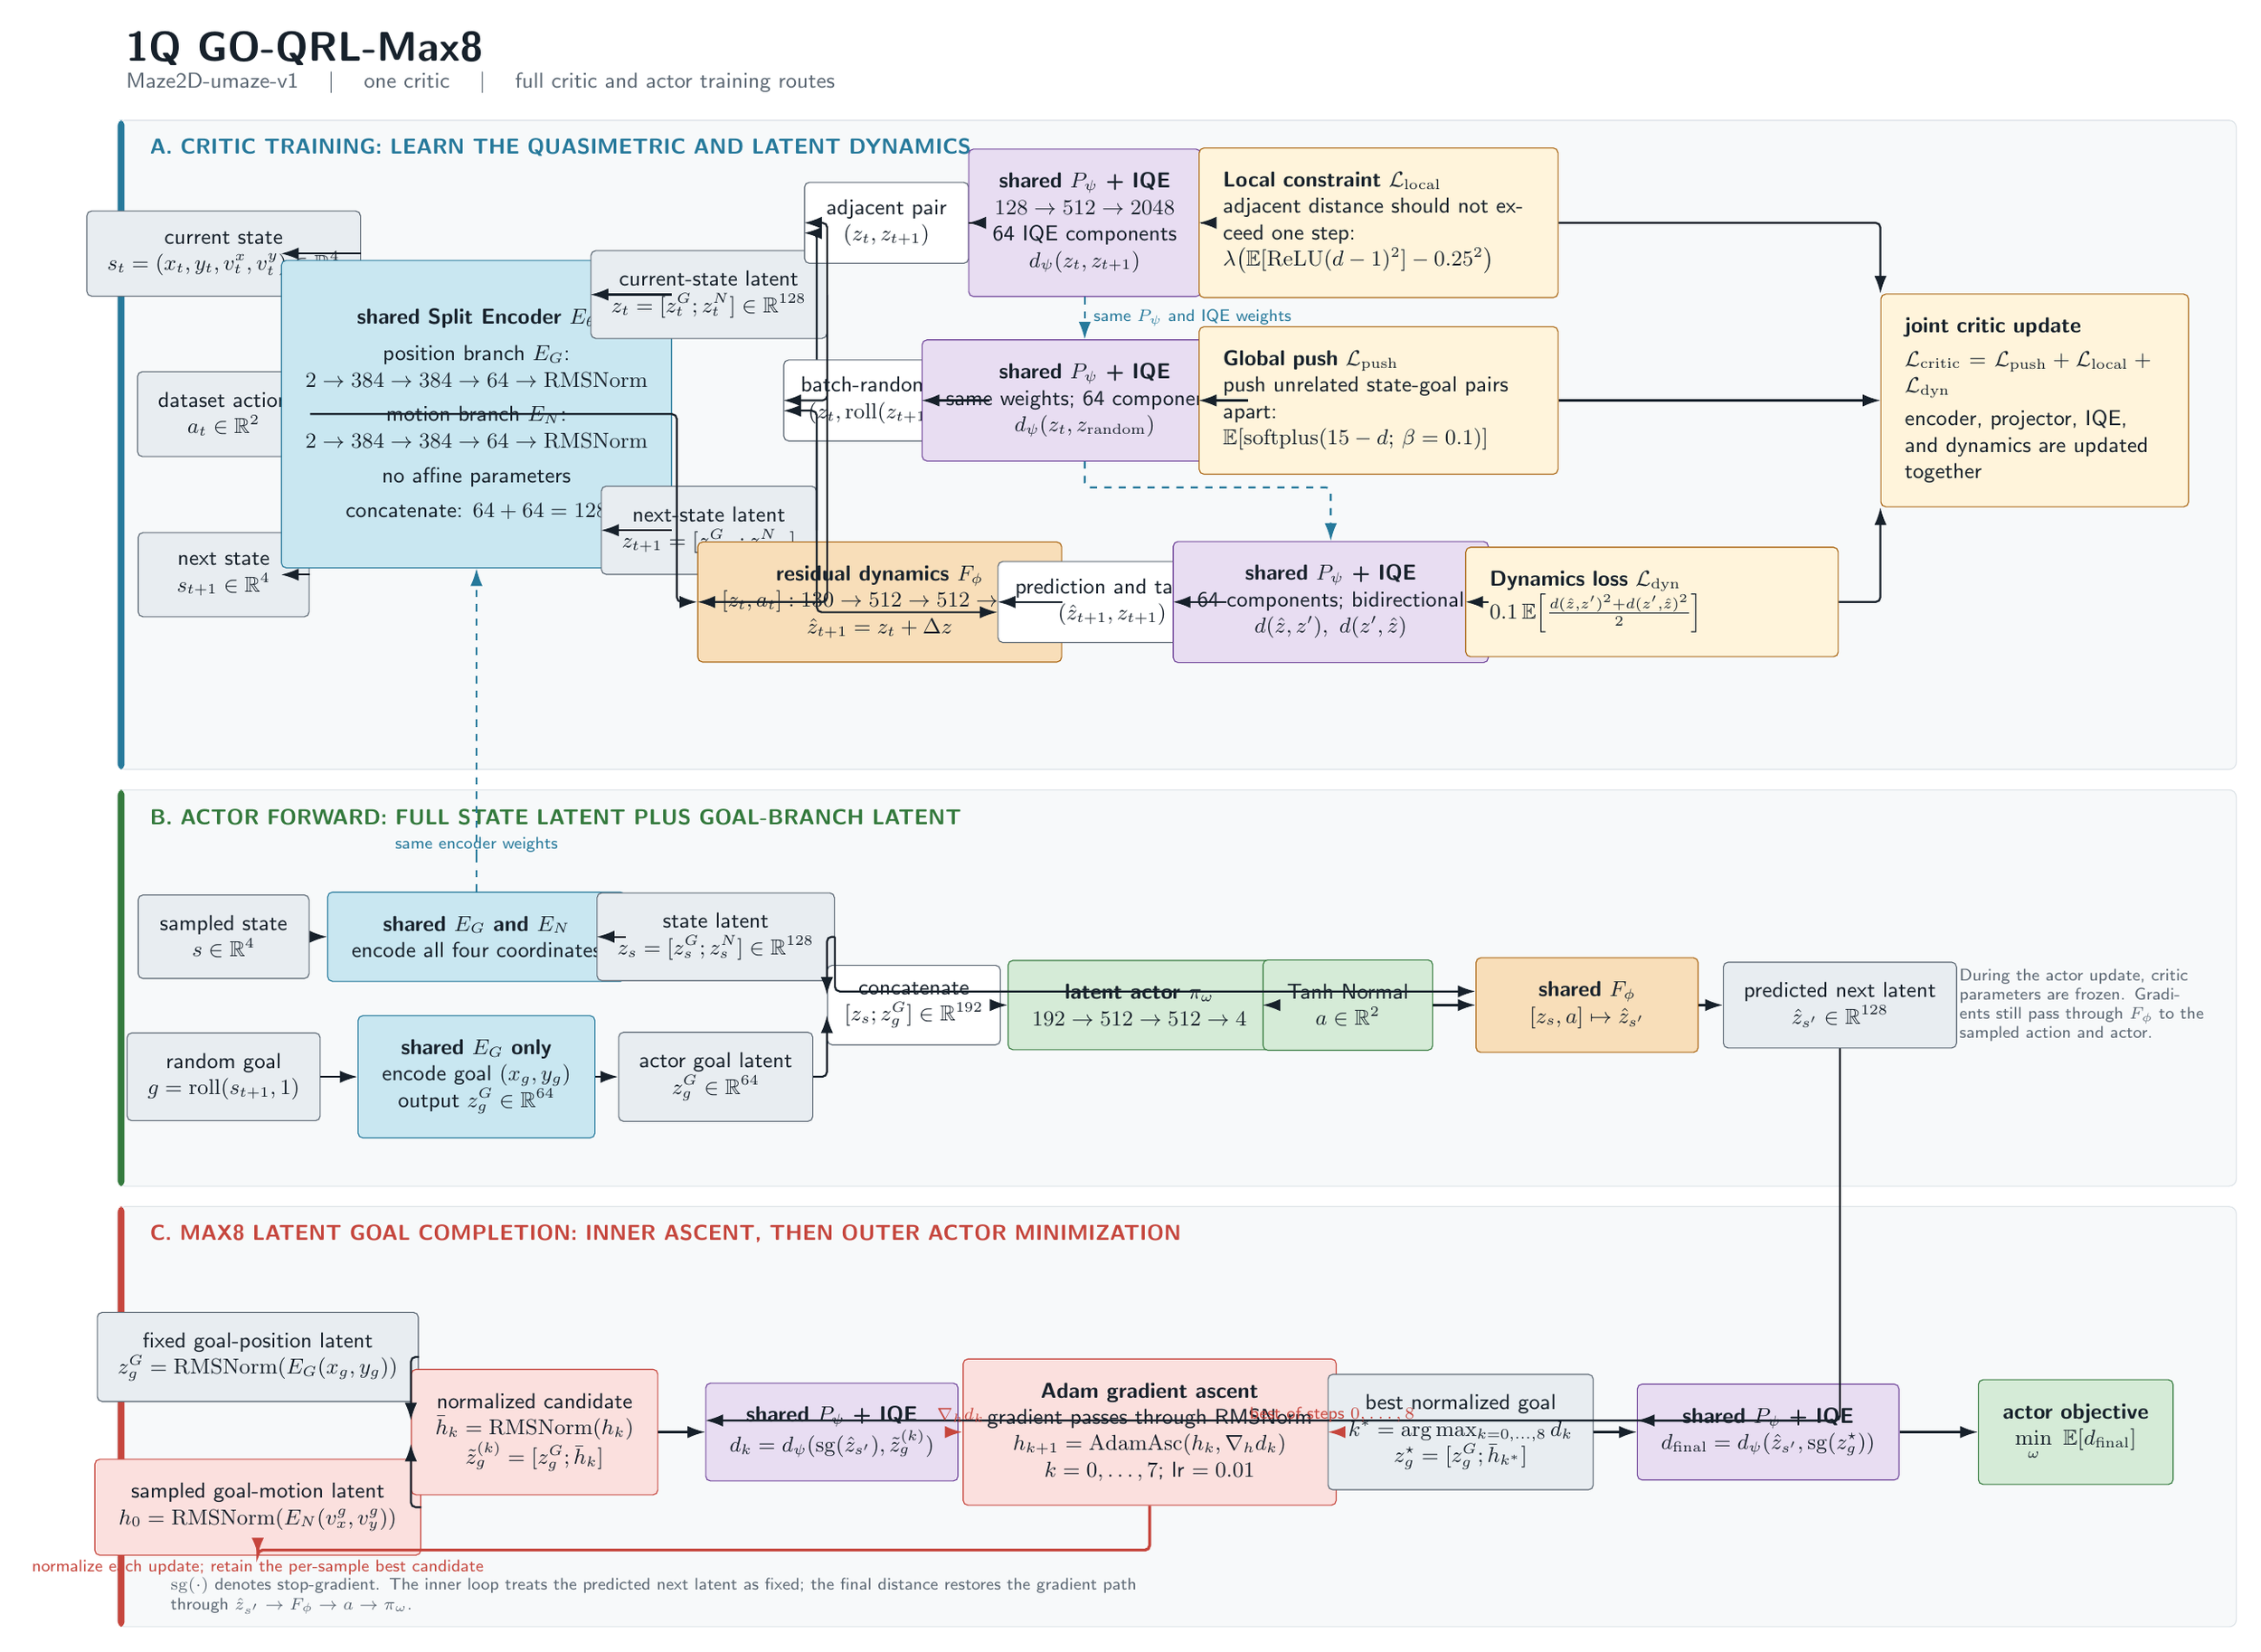
\begin{tikzpicture}[x=1cm,y=1cm]
  % Background swimlanes.
  \begin{scope}[on background layer]
    \filldraw[fill=panel, draw=panelborder, rounded corners=3pt]
      (0,-1.05) rectangle (31,-10.55);
    \filldraw[fill=panel, draw=panelborder, rounded corners=3pt]
      (0,-10.85) rectangle (31,-16.65);
    \filldraw[fill=panel, draw=panelborder, rounded corners=3pt]
      (0,-16.95) rectangle (31,-23.10);
    \fill[encoderline, rounded corners=2pt] (0,-1.05) rectangle (0.10,-10.55);
    \fill[actorline, rounded corners=2pt] (0,-10.85) rectangle (0.10,-16.65);
    \fill[loopline, rounded corners=2pt] (0,-16.95) rectangle (0.10,-23.10);
  \end{scope}

  % Header.
  \node[anchor=west, font=\sffamily\bfseries\LARGE] at (0,0)
    {1Q GO-QRL-Max8};
  \node[anchor=west, font=\sffamily\small, text=muted] at (0,-0.50)
    {Maze2D-umaze-v1 \quad $\vert$ \quad one critic \quad $\vert$ \quad full critic and actor training routes};

  % -----------------------------------------------------------------------
  % Critic route.
  \node[lane title, text=encoderline] at (0.35,-1.45)
    {A. CRITIC TRAINING: LEARN THE QUASIMETRIC AND LATENT DYNAMICS};

  \node[data, minimum width=2.5cm] (state) at (1.55,-3.00)
    {current state\\$s_t=(x_t,y_t,v^x_t,v^y_t)\in\mathbb{R}^4$};
  \node[data, minimum width=2.5cm] (logged-action) at (1.55,-5.35)
    {dataset action\\$a_t\in\mathbb{R}^2$};
  \node[data, minimum width=2.5cm] (next-state) at (1.55,-7.70)
    {next state\\$s_{t+1}\in\mathbb{R}^4$};

  \node[encoder, minimum width=4.4cm, minimum height=4.5cm] (split-encoder) at (5.25,-5.35) {
    \textbf{shared Split Encoder $E_\theta$}\\[1.5mm]
    position branch $E_G$:\\
    $2\rightarrow384\rightarrow384\rightarrow64\rightarrow\operatorname{RMSNorm}$\\[1.2mm]
    motion branch $E_N$:\\
    $2\rightarrow384\rightarrow384\rightarrow64\rightarrow\operatorname{RMSNorm}$\\[1.2mm]
    no affine parameters\\[1.2mm]
    concatenate: $64+64=128$
  };
  \node[data, minimum width=2.75cm] (current-latent) at (8.65,-3.60)
    {current-state latent\\$z_t=[z_t^G;z_t^N]\in\mathbb{R}^{128}$};
  \node[data, minimum width=2.75cm] (next-latent) at (8.65,-7.05)
    {next-state latent\\$z_{t+1}=[z_{t+1}^G;z_{t+1}^N]$};

  \draw[route] (state.east) -- (split-encoder.west |- state.east);
  \draw[route] (next-state.east) -- (split-encoder.west |- next-state.east);
  \draw[route] (split-encoder.east |- current-latent.west) -- (current-latent.west);
  \draw[route] (split-encoder.east |- next-latent.west) -- (next-latent.west);

  % Local constraint branch.
  \node[pair, minimum width=2.4cm] (local-pair) at (11.25,-2.55)
    {adjacent pair\\$(z_t,z_{t+1})$};
  \node[metric, minimum width=3.0cm] (local-metric) at (14.15,-2.55)
    {\textbf{shared $P_\psi$ + IQE}\\$128\to512\to2048$\\64 IQE components\\$d_\psi(z_t,z_{t+1})$};
  \node[loss, text width=4.55cm] (local-loss) at (18.45,-2.55) {
    \textbf{Local constraint $\mathcal L_{\rm local}$}\\
    adjacent distance should not exceed one step:\\
    $\lambda\!\left(\mathbb E[\operatorname{ReLU}(d-1)^2]-0.25^2\right)$
  };
  \draw[route] (current-latent.east) |- (local-pair.west);
  \draw[route] (next-latent.east) |- ([yshift=-1.5mm]local-pair.west);
  \draw[route] (local-pair.east) -- (local-metric.west);
  \draw[route] (local-metric.east) -- (local-loss.west);

  % Global push branch.
  \node[pair, minimum width=2.65cm] (global-pair) at (11.25,-5.15)
    {batch-random pair\\$(z_t,\operatorname{roll}(z_{t+1},1))$};
  \node[metric, minimum width=3.0cm] (global-metric) at (14.15,-5.15)
    {\textbf{shared $P_\psi$ + IQE}\\same weights; 64 components\\$d_\psi(z_t,z_{\rm random})$};
  \node[loss, text width=4.55cm] (global-loss) at (18.45,-5.15) {
    \textbf{Global push $\mathcal L_{\rm push}$}\\
    push unrelated state-goal pairs apart:\\
    $\mathbb E[\operatorname{softplus}(15-d;\,\beta=0.1)]$
  };
  \draw[route] (current-latent.east) |- (global-pair.west);
  \draw[route] (next-latent.east) |- ([yshift=-1.5mm]global-pair.west);
  \draw[route] (global-pair.east) -- (global-metric.west);
  \draw[route] (global-metric.east) -- (global-loss.west);

  % Latent dynamics branch.
  \node[dynamics, minimum width=3.25cm] (critic-dynamics) at (11.15,-8.10)
    {\textbf{residual dynamics $F_\phi$}\\
     $[z_t,a_t]:130\to512\to512\to128$\\
     $\hat z_{t+1}=z_t+\Delta z$};
  \node[pair, minimum width=2.6cm] (dynamics-pair) at (14.55,-8.10)
    {prediction and target\\$(\hat z_{t+1},z_{t+1})$};
  \node[metric, minimum width=3.0cm] (dynamics-metric) at (17.75,-8.10)
    {\textbf{shared $P_\psi$ + IQE}\\64 components; bidirectional\\$d(\hat z,z'),\ d(z',\hat z)$};
  \node[loss, text width=4.75cm] (dynamics-loss) at (22.45,-8.10) {
    \textbf{Dynamics loss $\mathcal L_{\rm dyn}$}\\
    $0.1\,\mathbb E\!\left[\frac{d(\hat z,z')^2+d(z',\hat z)^2}{2}\right]$
  };
  \draw[route] (current-latent.east) |- (critic-dynamics.west);
  \draw[route] (logged-action.east) -| ([xshift=-3mm]critic-dynamics.west) -- (critic-dynamics.west);
  \draw[route] (critic-dynamics.east) -- (dynamics-pair.west);
  \draw[route] (next-latent.east) |- ([yshift=-1.5mm]dynamics-pair.west);
  \draw[route] (dynamics-pair.east) -- (dynamics-metric.west);
  \draw[route] (dynamics-metric.east) -- (dynamics-loss.west);

  % Combined critic objective.
  \node[loss, text width=3.8cm, minimum height=3.0cm] (critic-total) at (28.05,-5.15) {
    \textbf{joint critic update}\\[1mm]
    $\mathcal L_{\rm critic}=
      \mathcal L_{\rm push}+
      \mathcal L_{\rm local}+
      \mathcal L_{\rm dyn}$\\[1mm]
    encoder, projector, IQE, and dynamics are updated together
  };
  \draw[route] (local-loss.east) -| (critic-total.north west);
  \draw[route] (global-loss.east) -- (critic-total.west);
  \draw[route] (dynamics-loss.east) -| (critic-total.south west);
  \draw[shared route] (local-metric.south) -- (global-metric.north)
    node[midway, right, note, text=encoderline] {same $P_\psi$ and IQE weights};
  \draw[shared route] (global-metric.south) -- ++(0,-0.38) -| (dynamics-metric.north);

  % -----------------------------------------------------------------------
  % Actor route.
  \node[lane title, text=actorline] at (0.35,-11.25)
    {B. ACTOR FORWARD: FULL STATE LATENT PLUS GOAL-BRANCH LATENT};
  \node[data, minimum width=2.5cm] (actor-state) at (1.55,-13.00)
    {sampled state\\$s\in\mathbb R^4$};
  \node[data, minimum width=2.5cm] (actor-goal) at (1.55,-15.05)
    {random goal\\$g=\operatorname{roll}(s_{t+1},1)$};
  \node[encoder, minimum width=3.15cm] (actor-state-enc) at (5.25,-13.00)
    {\textbf{shared $E_G$ and $E_N$}\\encode all four coordinates};
  \node[encoder, minimum width=3.15cm] (actor-goal-enc) at (5.25,-15.05)
    {\textbf{shared $E_G$ only}\\encode goal $(x_g,y_g)$\\output $z_g^G\in\mathbb R^{64}$};
  \node[data, minimum width=2.7cm] (actor-state-z) at (8.75,-13.00)
    {state latent\\$z_s=[z_s^G;z_s^N]\in\mathbb R^{128}$};
  \node[data, minimum width=2.7cm] (actor-goal-z) at (8.75,-15.05)
    {actor goal latent\\$z_g^G\in\mathbb R^{64}$};
  \node[pair, minimum width=2.2cm] (actor-input) at (11.65,-14.00)
    {concatenate\\$[z_s;z_g^G]\in\mathbb R^{192}$};
  \node[actor, minimum width=3.0cm] (actor-net) at (14.95,-14.00)
    {\textbf{latent actor $\pi_\omega$}\\$192\to512\to512\to4$};
  \node[actor, minimum width=2.15cm] (actor-dist) at (18.00,-14.00)
    {Tanh Normal\\$a\in\mathbb R^2$};
  \node[dynamics, minimum width=3.25cm] (actor-dynamics) at (21.50,-14.00)
    {\textbf{shared $F_\phi$}\\$[z_s,a]\mapsto\hat z_{s'}$};
  \node[data, minimum width=2.75cm] (predicted-z) at (25.20,-14.00)
    {predicted next latent\\$\hat z_{s'}\in\mathbb R^{128}$};
  \node[note, text width=3.6cm] at (28.75,-14.00)
    {During the actor update, critic parameters are frozen. Gradients still pass through $F_\phi$ to the sampled action and actor.};

  \draw[route] (actor-state.east) -- (actor-state-enc.west);
  \draw[route] (actor-goal.east) -- (actor-goal-enc.west);
  \draw[route] (actor-state-enc.east) -- (actor-state-z.west);
  \draw[route] (actor-goal-enc.east) -- (actor-goal-z.west);
  \draw[route] (actor-state-z.east) -| ([yshift=1.5mm]actor-input.west);
  \draw[route] (actor-goal-z.east) -| ([yshift=-1.5mm]actor-input.west);
  \draw[route] (actor-input.east) -- (actor-net.west);
  \draw[route] (actor-net.east) -- (actor-dist.west);
  \draw[route] (actor-dist.east) -- (actor-dynamics.west);
  \draw[route] (actor-state-z.east) |- ([yshift=2mm]actor-dynamics.west);
  \draw[route] (actor-dynamics.east) -- (predicted-z.west);
  \draw[shared route] (actor-state-enc.north) |- ++(0,0.45) -| (split-encoder.south)
    node[pos=0.15, above, note, text=encoderline] {same encoder weights};

  % -----------------------------------------------------------------------
  % Latent completion route.
  \node[lane title, text=loopline] at (0.35,-17.35)
    {C. MAX8 LATENT GOAL COMPLETION: INNER ASCENT, THEN OUTER ACTOR MINIMIZATION};
  \node[data, minimum width=2.7cm] (goal-position) at (2.05,-19.15)
    {fixed goal-position latent\\$z_g^G=\operatorname{RMSNorm}(E_G(x_g,y_g))$};
  \node[loop, minimum width=2.7cm] (free-motion) at (2.05,-21.35)
    {sampled goal-motion latent\\$h_0=\operatorname{RMSNorm}(E_N(v_x^g,v_y^g))$};
  \node[loop, minimum width=3.25cm] (candidate-goal) at (6.10,-20.25)
    {normalized candidate\\$\bar h_k=\operatorname{RMSNorm}(h_k)$\\$\tilde z_g^{(k)}=[z_g^G;\bar h_k]$};
  \node[metric, minimum width=3.45cm] (inner-metric) at (10.45,-20.25)
    {\textbf{shared $P_\psi$ + IQE}\\$d_k=d_\psi(\operatorname{sg}(\hat z_{s'}),\tilde z_g^{(k)})$};
  \node[loop, minimum width=3.65cm] (adam-ascent) at (15.10,-20.25)
    {\textbf{Adam gradient ascent}\\
     gradient passes through RMSNorm\\
     $h_{k+1}=\operatorname{AdamAsc}(h_k,\nabla_h d_k)$\\
     $k=0,\ldots,7$; lr $=0.01$};
  \node[data, minimum width=3.1cm] (completed-goal) at (19.65,-20.25)
    {best normalized goal\\$k^*=\arg\max_{k=0,\ldots,8}d_k$\\$z_g^\star=[z_g^G;\bar h_{k^*}]$};
  \node[metric, minimum width=3.5cm] (outer-metric) at (24.15,-20.25)
    {\textbf{shared $P_\psi$ + IQE}\\
     $d_{\rm final}=d_\psi(\hat z_{s'},\operatorname{sg}(z_g^\star))$};
  \node[actor, minimum width=2.85cm] (actor-loss) at (28.65,-20.25)
    {\textbf{actor objective}\\$\displaystyle\min_\omega\ \mathbb E[d_{\rm final}]$};

  \draw[route] (goal-position.east) -| ([yshift=1.7mm]candidate-goal.west);
  \draw[route] (free-motion.east) -| ([yshift=-1.7mm]candidate-goal.west);
  \draw[route] (candidate-goal.east) -- (inner-metric.west);
  \draw[route] (predicted-z.south) |- ([yshift=1.7mm]inner-metric.west);
  \draw[inner route] (inner-metric.east) -- (adam-ascent.west)
    node[midway, above, note, text=loopline] {$\nabla_h d_k$};
  \draw[inner route] (adam-ascent.south) -- ++(0,-0.65) -| (free-motion.south)
    node[pos=0.55, below, note, text=loopline] {normalize each update; retain the per-sample best candidate};
  \draw[inner route] (adam-ascent.east) -- (completed-goal.west)
    node[midway, above, note, text=loopline] {best of steps $0,\ldots,8$};
  \draw[route] (completed-goal.east) -- (outer-metric.west);
  \draw[route] (predicted-z.south) |- ([yshift=1.7mm]outer-metric.west);
  \draw[route] (outer-metric.east) -- (actor-loss.west);

  \node[note, anchor=west, text width=15cm] at (0.65,-22.65) {
    $\operatorname{sg}(\cdot)$ denotes stop-gradient. The inner loop treats the predicted next latent as fixed;
    the final distance restores the gradient path through $\hat z_{s'}\rightarrow F_\phi\rightarrow a\rightarrow\pi_\omega$.
  };
\end{tikzpicture}
\end{document}
